%%
%% IntegerLab (c) 2018-22 Christopher A. Bohn
%%
%% Licensed under the Apache License, Version 2.0 (the "License");
%% you may not use this file except in compliance with the License.
%% You may obtain a copy of the License at
%%     http://www.apache.org/licenses/LICENSE-2.0
%% Unless required by applicable law or agreed to in writing, software
%% distributed under the License is distributed on an "AS IS" BASIS,
%% WITHOUT WARRANTIES OR CONDITIONS OF ANY KIND, either express or implied.
%% See the License for the specific language governing permissions and
%% limitations under the License.
%%

%%
%% (c) 2021 Christopher A. Bohn
%%

\documentclass[12pt]{article}

\usepackage{fullpage}
\usepackage{fancyhdr}
\usepackage[procnames]{listings}
\usepackage{hyperref}
\usepackage{textcomp}
\usepackage{bold-extra}
\usepackage[dvipsnames]{xcolor}
\usepackage{etoolbox}


% Customize the semester (or quarter) and the course number

\newcommand{\courseterm}{Spring 2022}
\newcommand{\coursenumber}{CSCE 231}

% Customize how a typical lab will be managed;
% you can always use \renewcommand for one-offs

\newcommand{\runtimeenvironment}{your account on the \textit{csce.unl.edu} Linux server}
\newcommand{\filesource}{Canvas or {\footnotesize$\sim$}cse231 on \textit{csce.unl.edu}}
\newcommand{\filesubmission}{Canvas}

% These are placeholder commands and will be renewed in each lab

\newcommand{\labnumber}{}
\newcommand{\labname}{Lab \labnumber\ Assignment}
\newcommand{\shortlabname}{}
\newcommand{\duedate}{}

% Individual or team effort

\newcommand{\individualeffort}{This is an individual-effort project. You may discuss concepts and syntax with other students, but you may discuss solutions only with the professor and the TAs. Sharing code with or copying code from another student or the internet is prohibited.}
\newcommand{\teameffort}{This is a team-effort project. You may discuss concepts and syntax with other students, but you may discuss solutions only with your assigned partner(s), the professor, and the TAs. Sharing code with or copying code from a student who is not on your team, or from the internet, is prohibited.}
\newcommand{\freecollaboration}{In addition to the professor and the TAs, you may freely seek help on this assignment from other students.}
\newcommand{\collaborationrules}{}

% Do you care about software engineering?

\providebool{allowspaghetticode}

\setbool{allowspaghetticode}{false}

\newcommand{\softwareengineeringfrontmatter}{
    \ifboolexpe{not bool{allowspaghetticode}}{
        \section*{No Spaghetti Code Allowed}
        In the interest of keeping your code readable, you may \textit{not} use
        any \lstinline{goto} statements, nor may you use any \lstinline{break}
        statements to exit from a loop, nor may you have any functions
        \lstinline{return} from within a loop.
    }{}
}

\newcommand{\spaghetticodepenalties}[1]{
    \ifboolexpe{not bool{allowspaghetticode}}{
        \penaltyitem{1}{for each \lstinline{goto} statement, \lstinline{break}
            statement used to exit from a loop, or \lstinline{return} statement
            that occurs within a loop.}
    }{}
}

% You shouldn't need to customize these,
% but you can if you like

\lstset{language=C, tabsize=4, upquote=true, basicstyle=\ttfamily}
\newcommand{\function}[1]{\textbf{\lstinline{#1}}}
\setlength{\headsep}{0.7cm}
\hypersetup{colorlinks=true}

\newcommand{\startdocument}{
    \pagestyle{fancy}
    \fancyhf{}
    \lhead{\coursenumber}
    \chead{\ Lab \labnumber: \labname}
    \rhead{\courseterm}
    \cfoot{\shortlabname-\thepage}

	\begin{document}
	\title{\ Lab \labnumber}
	\author{\labname}
	\date{Due: \duedate}
	\maketitle

    \textit{\collaborationrules}
}

\newcommand{\rubricitem}[2]{\item[\underline{\hspace{1cm}} +#1] #2}
\newcommand{\bonusitem}[2]{\item[\underline{\hspace{1cm}} Bonus +#1] #2}
\newcommand{\penaltyitem}[2]{\item[\underline{\hspace{1cm}} -#1] #2}

%%
%% labs/common/semester.tex
%% (c) 2021-22 Christopher A. Bohn
%%
%% Licensed under the Apache License, Version 2.0 (the "License");
%% you may not use this file except in compliance with the License.
%% You may obtain a copy of the License at
%%     http://www.apache.org/licenses/LICENSE-2.0
%% Unless required by applicable law or agreed to in writing, software
%% distributed under the License is distributed on an "AS IS" BASIS,
%% WITHOUT WARRANTIES OR CONDITIONS OF ANY KIND, either express or implied.
%% See the License for the specific language governing permissions and
%% limitations under the License.
%%


% Customize the semester (or quarter) and the course number

\newcommand{\courseterm}{Fall 2022}
\newcommand{\coursenumber}{CSCE 231}

% Customize how a typical lab will be managed;
% you can always use \renewcommand for one-offs

\newcommand{\runtimeenvironment}{your account on the \textit{csce.unl.edu} Linux server}
\newcommand{\filesource}{Canvas or {\footnotesize$\sim$}cse231 on \textit{csce.unl.edu}}
\newcommand{\filesubmission}{Canvas}

% Customize for the I/O lab hardware

\newcommand{\developmentboard}{Arduino Nano}
%\newcommand{\serialprotocol}{SPI}
\newcommand{\serialprotocol}{I2C}
%\newcommand{\displaymodule}{MAX7219digits}
%\newcommand{\displaymodule}{MAX7219matrix}
\newcommand{\displaymodule}{LCD1602}

\setbool{usedisplayfont}{true}

\newcommand{\obtaininghardware}{
    The EE Shop has prepared ``class kits'' for CSCE 231; your class kit costs \$30.
    The EE Shop is located at 122 Scott Engineering Center and is open M-F 7am-4pm. You do not need an appointment.
    You may pay at the window with cash, with a personal check, or with your NCard.
    The EE shop does \textit{not} accept credit cards.
}

% Update to reflect the CS2 course(s) at your institute

\newcommand{\cstwo}{CSCE~156, RAIK~184H, or SOFT~161}

% Do you care about software engineering?

\setbool{allowspaghetticode}{false}

% Which assignments are you using this semester, and when are they due?

\newcommand{\pokerlabnumber}{1}
\newcommand{\pokerlabcollaboration}{
    Sections~\ref{sec:connecting}, \ref{sec:terminology}, \ref{sec:gettingstarted}, \ref{subsec:typesofpokerhands}, and~\ref{subsec:studythecode}: \freecollaboration
    Sections~\ref{sec:completingcard} and~\ref{subsec:completepoker}: \individualeffort
}
\newcommand{\pokerlabdue}{Week of August 29, before the start of your lab section}

\newcommand{\keyboardlabnumber}{2}
\newcommand{\keyboardlabcollaboration}{\individualeffort}
\newcommand{\keyboardlabdue}{Week of January 31, before the start of your lab section}

\newcommand{\pointerlabnumber}{3}
\newcommand{\pointerlabcollaboration}{\individualeffort}
\newcommand{\pointerlabdue}{Week of February 7, before the start of your lab section}

\newcommand{\integerlabnumber}{4}
\newcommand{\integerlabcollaboration}{\individualeffort}
\newcommand{\integerlabdue}{Week of February 14, before the start of your lab section}

\newcommand{\floatlabnumber}{5}
\newcommand{\floatlabcollaboration}{\individualeffort}
\newcommand{\floatlabdue}{soon}

\newcommand{\addressinglabnumber}{6}
\newcommand{\addressinglabcollaboration}{\individualeffort}
\newcommand{\addressinglabdue}{Week of February 28, before the start of your lab section}

%bomblab was 7
%attacklab was 8

\newcommand{\pollinglabnumber}{9}
\newcommand{\pollinglabcollaboration}{\individualeffort}
\newcommand{\pollinglabdue}{Week of April 11, before the start of your lab section}
\newcommand{\pollinglabenvironment}{your \developmentboard-based class hardware kit}

\newcommand{\ioprelabnumber}{\pollinglabnumber-prelab}
\newcommand{\ioprelabcollaboration}{\freecollaboration}
\newcommand{\ioprelabdue}{Before the start of your lab section on April 5 or 6}

\newcommand{\interruptlabnumber}{10}
\newcommand{\interruptlabcollaboration}{\individualeffort}
\newcommand{\interruptlabdue}{Week of April 18, before the start of your lab section}
\newcommand{\interruptlabenvironment}{your \developmentboard-based class hardware kit}

\newcommand{\capstonelab}{ComboLock}    % this will come into play when we generalize capstonelab
\newcommand{\capstonelabnumber}{11}
\newcommand{\capstonelabcollaboration}{\teameffort}
\newcommand{\capstonelabdue}{Week of May 2, Before the start of your lab section\footnote{See Piazza for the due dates of teams with students from different lab sections.}}
\newcommand{\capstonelabenvironment}{your \developmentboard-based class hardware kit}

\newcommand{\memorylabnumber}{12}
\newcommand{\memorylabcollaboration}{This is an individual-effort project. You may discuss the nature of memory technologies and of memory hierarchies with classmates, but you must draw your own conclusions.}
\newcommand{\memorylabdue}{Week of May 2, at the end of your lab section}
\newcommand{\memorylabenvironment}{your \developmentboard-based class hardware kit and your account on the \textit{csce.unl.edu} Linux server}

% Labs not used this semester

\newcommand{\concurrencylabnumber}{XX}
\newcommand{\concurrencylabcollaboration}{\individualeffort}
\newcommand{\concurrencylabdue}{not this semester}

\newcommand{\ssbcwarmupnumber}{XX}
\newcommand{\ssbcwarmupcollaboration}{\freecollaboration}
\newcommand{\ssbcwarmupdue}{not this semester}

\newcommand{\ssbcpollingnumber}{XX}
\newcommand{\ssbcpollingcollaboration}{\individualeffort}
\newcommand{\ssbcpollingdue}{not this semester}

\newcommand{\ssbcinterruptnumber}{XX}
\newcommand{\ssbcinterruptcollaboration}{\individualeffort}
\newcommand{\ssbcinterruptdue}{not this semester}

%%
%% labs/common/storylines.tex
%% (c) 2020-23 Christopher A. Bohn
%%
%% Licensed under the Apache License, Version 2.0 (the "License");
%% you may not use this file except in compliance with the License.
%% You may obtain a copy of the License at
%%     http://www.apache.org/licenses/LICENSE-2.0
%% Unless required by applicable law or agreed to in writing, software
%% distributed under the License is distributed on an "AS IS" BASIS,
%% WITHOUT WARRANTIES OR CONDITIONS OF ANY KIND, either express or implied.
%% See the License for the specific language governing permissions and
%% limitations under the License.
%%

\newcommand{\MeetArchie}{
    \begin{wrapfigure}{r}{0.33\textwidth}
        \centering
        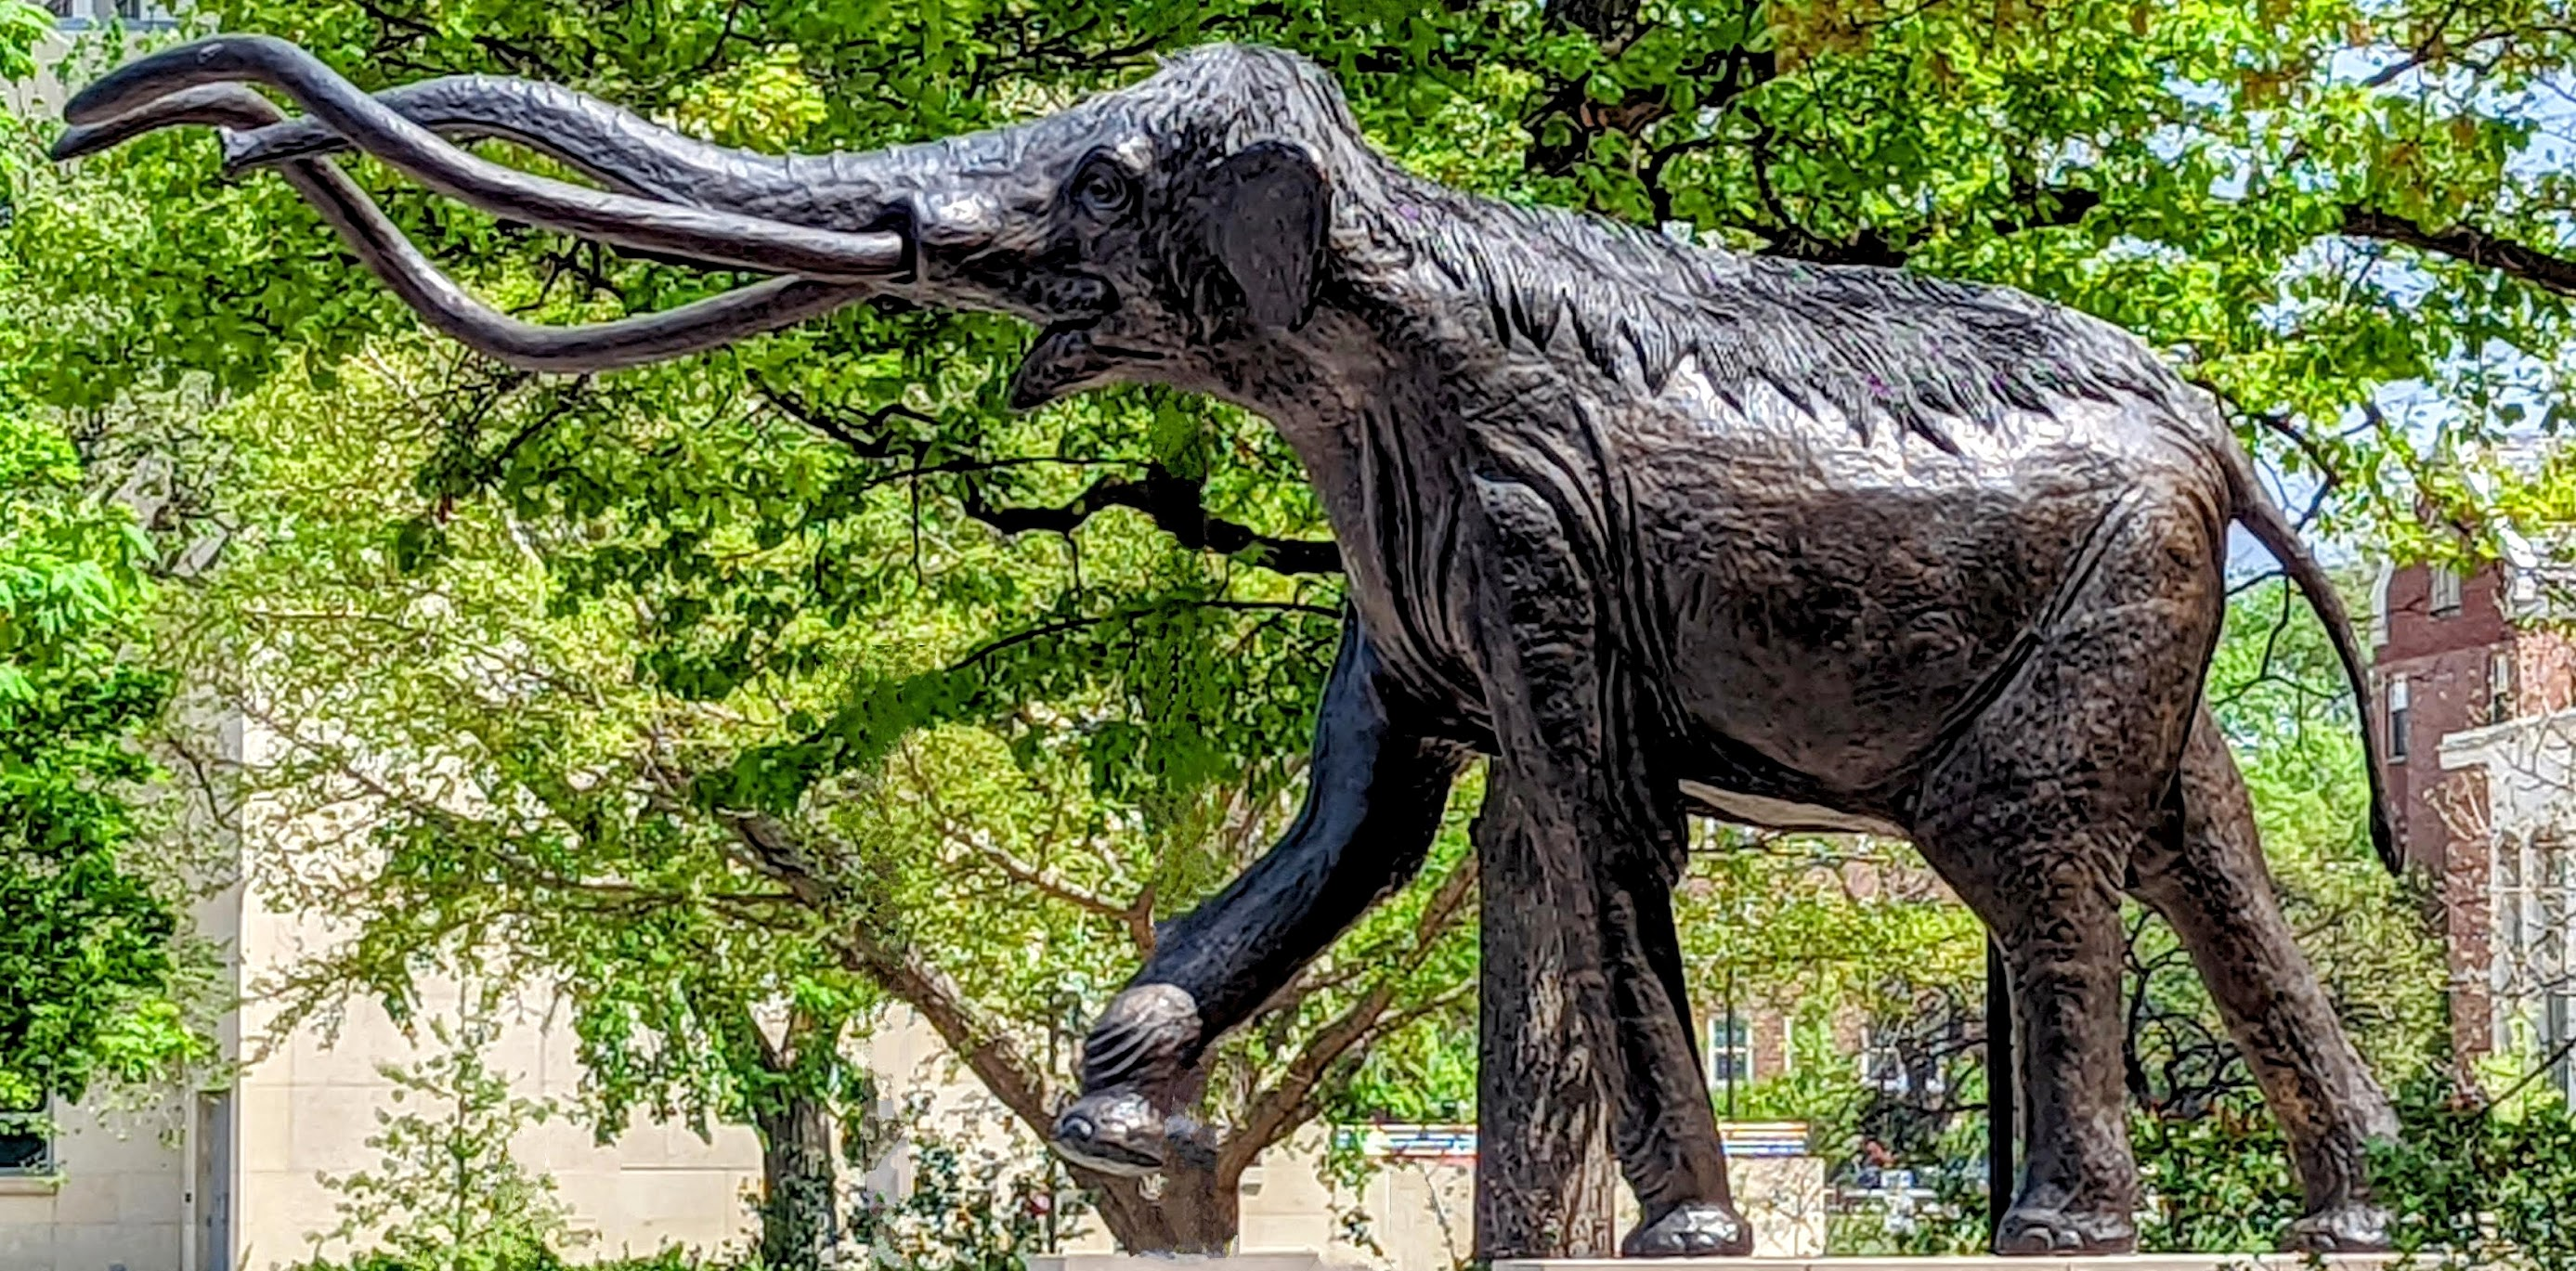
\includegraphics[width=.4\textwidth]{archie}
        \caption{Archie.\\ \footnotesize{Photograph by Bohn.}}
    \end{wrapfigure}

    You're relaxing at your favorite hangout when another customer catches your attention.
    He's rather large (dare I say, \textit{mammoth}), a bit hairy, and looking frustrated in front of his laptop.
    ``I'm Archie,'' he says, ``and I'm trying to teach myself this card game called \textit{Poker}.
    I found this source code that I thought I could use to understand Poker better, but the code is incomplete, and I don't entirely understand what's there.
    Could you explain the code to me, please?'
}

\newcommand{\GetHired}{
    Archie's face lights up in a very big smile.
    ``Thanks!''
    After pausing in thought for a moment, he says, ``Say, I've got a new startup company that could really use your help.
    Are you interested?
    It'll be exciting!''
}

\newcommand{\FirstDayOnTheJob}{
    \begin{wrapfigure}{r}{0.33\textwidth}
        \centering
        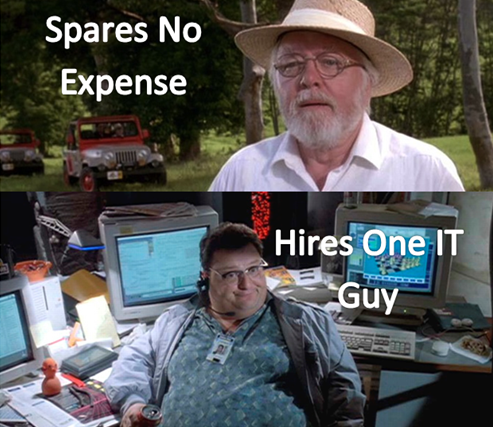
\includegraphics[width=.4\textwidth]{some-expenses-spared}
        \caption{Some expenses were spared.\\ \footnotesize{Original images \textcopyright\ Universal Studios and Amblin Entertainment, Inc. Meme creator unknown.}}
    \end{wrapfigure}

    You've recently been hired to help get the Pleistocene Petting Zoo get started.
    Your new employer, Archie, is surprisingly honest: he admits to you that some expenses were spared.
    Archie cheerfully points out that any challenge is also an opportunity to succeed.
    You suspect your job will offer plenty of ``opportunities to succeed.''
}

\newcommand{\HasKeyboard}{
    Great news!
    Archie brings you your new keyboard.
    He also brings you a problem of his own.
    Because you were held up with the broken keyboard, Archie decided to try some programming on his own, and his code is behaving strangely.
}

\newcommand{\ArchieWroteSmellyCode}{
    Working at the Pleistocene Petting Zoo certainly is proving to be interesting.
    You're glad that you don't have to worry about the problem of the giant sloths very slowly chasing their handlers, but now it seems that Archie has decided to try to write a program or two.
    At a glance, his code is smellier than the wooly rhinoceros' enclosure.
    But you take a closer look anyway to try to understand why his code acts strangely.
}

\newcommand{\InsurancePreview}{
    You hear somebody enter the room.
    ``\textit{Frankenstein}, `boat','' is the challenge, and she answers, ``borne.''
    Archie introduces you to the new arrival, ``Lil, this is our new developer, the one who wrote the app we just used.''
    He turns to you: ``This is Lilith Redd from business operations.''
    He turns back to her and continues, ``Lil, what's the good word?''

    ``The word isn't good, I'm afraid.
    I just heard back from the insurance company.''
}

\newcommand{\OnLoanToEclecticElectronics}{
    All work at the Pleistocene Petting Zoo has stopped while Archie tries to find a $\cancelto{\mathrm{reasonable}}{\mathrm{gullible}}$ insurance company.
    Rather than furloughing staff, he's asked everybody to help out with his other startup companies for a week or two.
    He specifically asked that you help out with Eclectic Electronics.

    Herb Bee, the chief engineer, explains that Eclectic Electronics is developing a patent-pending C-licon tool that will convert C code into an integrated circuit that has the same functionality as the original C code.
    To test it out, he tasked you with writing the code to implement an Arithmetic Logic Unit (ALU).
    Your task will be to implement integer addition, subtraction, multiplication, and division.
    Even though high-level languages' \textit{logical} boolean operations normally are not part of an ALU, Herb wants you to include these in the ALU to see if that can make some programs run faster.
    Because bitwise operations and bit shift operations have been implemented, you will be able to use C's bitwise and bit shift operators, but because arithmetic operations have not yet been implemented, you cannot use C's arithmetic operators.
    Because C library functions generally make use of arithmetic operations (which have not yet been implemented), you cannot use library functions.
}

\newcommand{\SuccessfulALU}{
    Herb smiles as he hands you the the test results from the latest integrated circuit fab batch.
    ``C-licon successfully turned your code into an ALU.
    Nicely done!''
    I think maybe it's time to use C-licon to see if we can improve the Floating Point Unit (FPU) on our experimental microprocessor.
}

\newcommand{\WriteAnFPU}{
    Herb tells you that, Eclectic Electronics tested the integrated circuit that the C-licon tool created from your ALU code, and they've concluded that C-licon is ready to use for their new experimental microprocessor.
    He tasks you with writing C code (that will be used by the C-licon tool) to implement a Floating Point Unit (FPU).
    Your task will be to implement floating point addition, subtraction, multiplication, and division.
    You can use any bit operations and, thanks to the ALU you wrote, you can use any integer arithmetic operations (use the conventional + - * / operators).
    Because the FPU has not yet been implemented, you cannot use C's floating point operations, you cannot use \lstinline{float}s nor \lstinline{double}s, and you cannot use library functions.
}

\newcommand{\GoingBackToTheZoo}{
    Lil enters the room.
    Herb challenges her: ``\textit{Gulliver's Travels}, `endian','' and Lil answers, ``ends.''

    Lil walks up to you and says, ``We have the insurance situation taken care of, and it's time to get the Zoo ready for guests.
    We're reassembling the tech team, and there's plenty of work to do.''

    You smile.
    ``That's good news!''

    Lil's face is hard to read.
    ``Well, yes and no.
    It's good that you'll be able to resume work on the Zoo's systems.
    But while Archie was waiting for us to fix the insurance situation, he got bored and -- cutting a long story short -- he ended up creating some new `opportunities' that we need you `to succeed' at.''
}

\newcommand{\SettledIntoRoutine}{
    You've settled into a comfortable routine at the Pleistocene Petting Zoo.
    While your job isn't quite as exciting as that of the saber-toothed tigers' dentist, it still has something new and interesting almost every day.

    Archie announces that he heard that hand-crafted assembly code can be faster than high-level language code.
    You try to explain that while this may have been true decades ago, modern optimizing compilers generate code faster than what a typical programmer can achieve with assembly code.
    Archie doesn't believe you and insists that you write the zoo's new cipher program in x86 assembly code.
}

\newcommand{\NewmanRanOffWithSamples}{
    Archie is hurriedly packing is trunk, like he's about to leave on a short-notice urgent trip.
    Before charging out the door, he pauses to tell you, ``Newman just stole some of our samples.
    I need to track him down before he sells them to the Supersized Safari Syndicate.
    I guess this means you're in charge of the Zoo's computer system now.
    Don't worry, you'll be fine. What could possibly go wrong?''
}

\newcommand{\BombLabIntroduction}{  % Ties Bryant & O'Halloran's Bomb Lab into the Pleistocene Petting Zoo story
    In a jarring collision of movie franchises, the CEO of Virtucon makes a Zoom call to the Pleistocene Petting Zoo.
    For some reason that nobody really explains, you're the only person available to handle the situation.
    The guy, who sounds kind of like an animated ogre, demands that the Pleistocene Petting Zoo deliver to him a megalodon shark with a head-mounted laser capable of emitting a beam of pure antimatter.

    You blurt out, ``Then it's not a laser,'' and then try to explain to him that megalodons are from the Miocene epoch, and expecting to find them at the Pleistocene Petting Zoo would be as ridiculous as a Cretaceous-period tyrannosaur at a Jurassic-themed park.

    ``Zip it!'' commands the guy who kind of looks like the host of a public-access show you used to watch.
    ``Since you won't meet my demand, my minions have placed a `binary bomb' under your zoo.
    Because I like really convoluted plans, we put software on your Linux server that controls the bomb.
    If you do nothing, the bomb will explode.
    If you turn off the Linux server, the bomb will explode.
    If you go slower than 50mph, the bomb will -- no, never mind that last part.

    ``The bomb software consists of a sequence of phases.
    Each phase expects you to type a particular string on \texttt{stdin}.
    If you type the correct string, then the phase is {\em defused} and the bomb proceeds to the next phase. Otherwise, the bomb {\em explodes}.
    The bomb is defused when every phase has been defused.

    ``Your mission, which you have no choice but to accept, is to defuse your bomb before the due date.
    Good luck, and welcome to the bomb squad!''
}

\newcommand{\FoodLockersAreStuck}{
    Having saved the Zoo from Dr. Evil's binary bomb, you relax back in your chair and think about taking a break.
%SPRINGBREAK
    Maybe an entire week in which you don't have solve any problems or meet any deadlines -- that'd be real nice.
%FALLBREAK
    % Maybe 4-day weekend in which you don't have solve any problems or meet any deadlines -- that'd be real nice.

    Another Zoom call comes in.
    \textit{What now!?} you wonder as you take your feet off of the desk to answer the call.
    An uncomfortable-looking animal handler says, ``We can't unlock the food lockers.
    It's the animals' feeding time, and we can't open the food lockers!
    It's feeding time, we can't get to the animals' food, and,'' his eyes dart nervously toward the animal enclosures, ``and many of them have sharp, pointy claws and others have big, stompy feet.''
}

\newcommand{\AttackLabIntroduction}{    % Ties Bryant & O'Halloran's Attack Lab into the Pleistocene Petting Zoo story
    You managed to keep the Pleistocene Petting Zoo from blowing to smithereens, but it turns out that Dr. Evil's minions weren't too careful when they put the bomb control software on the Zoo's Linux server.
    The software that controls the food locker has been heavily damaged!
    The functions that unlock the food locker doors are still present, but there's no way to activate those functions.

    You then recall what Archie told you when he hired you: some expenses were spared.
    You run the machine code through a disassembler and quickly see that it has a buffer overflow vulnerability.
    Before the situation in the dire wolf enclosure gets too dire, you sit down and get to work.

    The \function{ctarget} code runs on an older machine that allows executable code to be present on the stack, so it's vulnerable to a conventional code injection buffer overflow attack.
    \begin{itemize}
        \item Phase 1 (\function{touch1}) unlocks the food locker so the animal handlers can prepare the food.
        \item Phase 2 (\function{touch2}) opens the doors between the food locker and the carnivore enclosures;
        you will need to pass a cookie to the function to authenticate yourself.
        \item Phase 3 (\function{touch3}) closes the doors between the food locker and the carnivore enclosures.
    \end{itemize}
    The \function{rtarget} code runs on a newer machine that does not allow executable code to be present on the stack, so you'll have to conduct a return-oriented programming attack on it.
    \begin{itemize}
        \item Phase 4 (\function{touch2)} opens the doors between the food locker and the herbivore enclosures;
        you will need to pass a cookie to the function to authenticate yourself.
        \item Phase 5 (\function{touch3}) closes the doors between the food locker and the herbivore enclosures.
    \end{itemize}
}

\newcommand{\MostAnimalsAreFed}{
    Before you take on the Phase 5, pause to consider what you have accomplished so far.
    In Phases 2 and 3, you caused a program to execute machine code of your own design.
    If {\sc ctarget} had been a network server, you could have injected your own code into a distant machine.
    In Phase 4, you circumvented two of the main devices modern systems use to thwart buffer overflow attacks.
    Although you did not inject your own code, you were able inject a type of program that operates by stitching together sequences of existing code.
    Also, all animals have been fed, the carnivores are still in their enclosure, the mammoths can't fit through the herbivore door, and only the giant sloths seem interested in very slowly escaping.
}

\newcommand{\ArchieReturns}{
    Archie returns from tracking down Newman, who'd run off with some of the Pleistocene Petting Zoo's samples shortly before Dr.~Evil's Zoom call.
    ``It turns out he didn't get very far at all,'' Archie sighs.
    ``He ran into a flock of terror birds as he was leaving, and we found him in one of the emergency shelters.

    Archie smiles. ``I trust things were uneventful while I was away?''
}

\newcommand{\PickingUpNewmansProject}{
    Archie seems genuinely surprised that Newman is refusing to go back to work.
    ``You would think that he'd be grateful for being rescued from that flock of terror birds.''
    Before you can wonder out-loud whether it would be a good idea to trust someone who had just tried to sell trade secrets to a competitor, Archie gives you your new task.

    ``Because Newman isn't cooperating, I need you to finish the project he was working on.
    As you can imagine, duplicating the genetic information for our exhibits can take a long time, and Newman realized that we might be able to duplicate the data faster if we had a concurrent program which has one thread reading from the original data and another thread writing the copy.
    Unfortunately, he ran off to sell samples to the  Supersized Safari Syndicate before finishing the duplicator.
    Right now the duplicator seems to work, but it usually makes imperfect copies.
    Have you ever seen a paleolama with two noses, four eyes, and no ears!?''
}

\newcommand{\WeNeedBetterDetection}{
    Between Newman trying to sell samples to a competitor, that weird guy almost blowing up the zoo, and the animals almost escaping, Archie is getting worried.
    ``I think we need to introduce additional protective measures.
    As useful as your challenge-response app is in helping us detect intruders, I think it's now clear that we need something that will detect someone -- or some\textit{thing} -- when they're someplace they shouldn't be, even when no one else is around.
    I've asked the team at Eclectic Electronics to put something together.''
}

\newcommand{\WeNeedBetterLocks}{
    Between Newman trying to sell samples to a competitor, that weird guy almost blowing up the zoo, and the animals almost escaping, Archie is getting worried.
    ``I think we need to introduce additional protective measures.
    As useful as your challenge-response app is in helping us detect intruders, I think it's now clear that we need something that will keep someone -- or some\textit{thing} -- out of places they shouldn't be, even when no one else is around.
    I've asked the team at Eclectic Electronics to put something together.''
}

\newcommand{\IntroduceHardware}{
    Archie walks up to you, along with Herb Bee from Eclectic Electronics.
    Herb is holding a tangled mess of electronics.
    Archie explains, ``Herb here has developed a prototype of a device that he thinks will be useful for our physical security needs, as well as a few other applications around here. He calls it the \textit{Cow Pi}.''

% TODO: parameterize based on which microcontroller is actually being used
    You look at the device in Herb's hands and see the \nano\ central to the circuit.
    ``Isn't \textit{-Pi} typically used as a suffix for circuits that use a Raspberry Pi instead of an Arduino?''

    Herb replies, ``Typically, yes, but \textit{Cowduino} isn't very punny, is it?''

    Archie chimes in, ``Maybe with the right emphasis: \textit{Cow-DOO-ino}.''

    ``That's kind of subtle, don't you think? How will people know to put the emPHAsis on that sylLAble?''

    ``I think we're getting off topic here,'' you point out.
    ``How can I help?''

    ``Oh, right,'' Herb says, ``We'd like you to kick its proverbial tires.
    Let's start off with something simple, like a number builder tool.''
}

\newcommand{\JeffGoldblum}{
    Herb looks over your work.
    ``Hmm, yes. I think this is coming along nicely.
    Let's run a few more tests.''

    Archie storms into the room.
    ``We have \textit{got} to do something about security!
    How's that doodad coming along?
    Because there's now a half-man/half-fly in the labs going on-and-on about Chaos Theory and how if we just give him a MacBook and a spaceship then he'll be able to get the Lord of Thunder to travel across the 8th Dimension.
    Is that thing just about ready?''

    Herb shakes his head, ``No, not quite yet. It should be ready in about a week.''
}

\newcommand{\DisdainfulHerb}{
    Smoke wafts from Herb's soldering iron as he looks up when you approach.
    Cleaning the iron's tip, he quotes:
    ``Somebody once said, `The three most dangerous things in the world are a programmer with a soldering iron, a hardware engineer with a software patch, and'{}'' -- he glances nervously in Archie's direction -- ``{}`a user with an idea.'\footnote{
        Rick Cook, \textit{The Wizardry Consulted}, 1995.
    }$^{\mathrm{,}}$\footnote{
        The notion of being wary of programmers wielding screwdrivers or soldering irons long pre-dated this quote, as there are apocryphal tales of people who found it easier to modify the hardware to suit the software rather than the other way around.
    }''
}

\newcommand{\NumberConversionTool}{     % Since we're now allowing `sprintf()` with the LCD1602, converting between decimal and hexadecimal is trivial; it still might be okay for 7-segment displays
    Herb gets straight to the point.
    ``We promised Archie that we'd be able to start using the Cow Pi to build systems in a week.
    So far we've tested its input/output functionality, but we still need to test its timer and also whether we can take inputs without constantly polling the input devices.
    As before, we don't need to do anything too fancy;
    let's try a number base conversion tool.''
}

\newcommand{\LessDisdainfulHerb}{
    Smoke wafts from Herb's soldering iron as he looks up when you approach.
    Cleaning the iron's tip, he notes:
    ``Somebody once said that one of the most dangerous things in the world is a programmer with a soldering iron.''\footnote{
        ``The three most dangerous things in the world are a programmer with a soldering iron, a hardware engineer with a software patch, and a user with an idea.'' -- Rick Cook, \textit{The Wizardry Consulted}, 1995.
    }$^{\mathrm{,}}$\footnote{
        The notion of being wary of programmers wielding screwdrivers or soldering irons long pre-dated this quote, as there are apocryphal tales of people who found it easier to modify the hardware to suit the software rather than the other way around.
    }
}

\newcommand{\RemoteControlledCar}{

    About this time, Archie walks by, thinking about electric carts to transport visitors around the Pleistocene Petting Zoo.
    ``They probably should be remote-controlled.''
    He looks at you and Herb, and asks, ``Do you think you could make a cart a remote-controlled cart?''

    You ask the obvious question, ``Are there carts here already?''

    Archie waves his hand in the air, dismissing that detail, ``Not yet, but could you make the remote-control?''
    
    You hestatingly summarize: ``You want a cartless remote-controlled cart?''

    Archie beamingly smiles, ``Exactly!''

    Herb jumps in, ``Yes, we'll do it.''
    Herb looks at you and adds, ``It'll give us a chance to test the Cow Pi's timer and whether we can take inputs without constantly polling the input devices.''
}

\newcommand{\LauraDern}{
    You and Herb look for Archie in the Pleistocene Petting Zoo's labs to give him the good news, and you find a blond woman wearing cargo shorts, butchering a Gilbert and Sullivan song\dots \\ \\
    \textmusicalnote\ I am the very model of a modern vice admiral \textmusicalnote \\
    \textmusicalnote\ I've information about all things paleobotanical \textmusicalnote \\
    \textmusicalnote\ And I've been up to my armpits in problems scatological \textmusicalnote \\
    \textmusicalnote\ During the regency I had experience matriarchical \textmusicalnote \\
    \textmusicalnote\ I plot space travel, normal and superluminal \textmusicalnote \\
    \textmusicalnote\ (Even if I challenge the Pauli exclusion principle) \textmusicalnote \\

    ``I don't know how these people keep getting into our labs.
    \textit{Please} tell me that you have good news,'' pleads Archie.

    ``Yes, the Cow Pi is ready for whatever you need: calculators, security systems, parking meters -- you name it,'' Herb cheerfully responds.

    ``Excellent.''
    Archie turns to you.
    ``I'd like you and Newm... no, \textit{not} Newman.
    I'd like you and someone else on the staff to get started right away.
    Here's what I'd like to have built first.''
}

\newcommand{\CalculatorNeeded}{
    ``I have various teams working on different projects around here to improve security,'' Archie reminds you.
    He glances toward the Zoo's labs, where there's now a guy who looks like the actor who portrayed the fictional actor who portrayed the Norse god Odin, trying to avoid children while wistfully talking about raising rabbits in Montana.
    You briefly wonder why there are children someplace where there are also carnivorous megafauna, and then you remember that you work at a petting zoo.
    ``What I need your team to do,'' Archie continues, ``is make a four-function calculator so that we can quickly and easily determine whether we have the correct number of specimens, or if any are missing.''
}

\newcommand{\CalculatorCounting}{
    Technicians are using your calculator to compute how many specimens are still present in the lab, and establish that all specimens are accounted for after Newman's attempted theft.
    As reports come in of facilities getting secured with Cow Pi-based locks and passages being monitored with Cow Pi-based motion sensors, Archie smiles and tells you that this was a job well done.
    With all of the excitement neatly wrapped-up and arriving at a satisfactory conclusion, you look forward to a boring career in which there's absolutely no screaming and running for your life.
}

\newcommand{\CombinationLockNeeded}{
    ``I have various teams working on different projects around here to improve security,'' Archie reminds you.
    He glances toward the Zoo's labs, where there's now a guy who looks like the actor who portrayed the fictional actor who portrayed the Norse god Odin, trying to avoid children while wistfully talking about raising rabbits in Montana.
    You briefly wonder why there are children someplace where there are also carnivorous megafauna, and then you remember that you work at a petting zoo.
    ``What I need your team to do,'' Archie continues, ``is make a combination lock so that only authorized people can get into our lab facilities.''
}

\newcommand{\CombinationLockInstalled}{
    After fastening the new electronic combination lock to the lab door, Archie smiles and tells you that this was a job well done.
    With all of the excitement neatly wrapped-up and arriving at a satisfactory conclusion, you look forward to a boring career in which there's absolutely no screaming and running for your life.
}

\newcommand{\RangeFinderNeeded}{
    ``I have various teams working on different projects around here to improve security,'' Archie reminds you.
    He glances toward the Zoo's labs, where there's now a guy who looks like the actor who portrayed the fictional actor who portrayed the Norse god Odin, trying to avoid children while wistfully talking about raising rabbits in Montana.
    You briefly wonder why there are children someplace where there are also carnivorous megafauna, and then you remember that you work at a petting zoo.
    ``What I need your team to do,'' Archie continues, ``is make a range finder that will alert us when someone -- or some\textit{thing} -- gets too close to someplace they shouldn't be.''
}

\newcommand{\RangeFinderDetecting} {
    A technician installing a new range finder outside the lab door briefly sets off the alarm, but then the range finder falls quiet and faithfully reports that nothing is approaching.
    As reports come in of facilities getting secured with Cow Pi-based locks, and of accurate speciment counts accomplished with Cow Pi-based calculators, Archie smiles and tells you that this was a job well done.
    With all of the excitement neatly wrapped-up and arriving at a satisfactory conclusion, you look forward to a boring career in which there's absolutely no screaming and running for your life.
}


\renewcommand{\labnumber}{\integerlabnumber}
\renewcommand{\labname}{Integer Representation and Arithmetic Lab}
\renewcommand{\shortlabname}{integerlab}
\renewcommand{\collaborationrules}{\integerlabcollaboration}
\renewcommand{\duedate}{\integerlabdue}

\pagelayout
\begin{document}
\labidentifier\

\pdfbookmark[1]{Frontmatter}{frontmatter}                                                               In this assignment, you will write code for \runtimeenvironment\ that will use new electronic devices to interact with the physical world.

The instructions are written assuming you will edit the code in the Arduino IDE and run it on \runtimeenvironment, constructed according to the pre-lab instructions.
If you wish, you may edit the code in a different environment; however, our ability to provide support for problems with other IDEs is limited.

\section*{Learning Objectives}

After successful completion of this assignment, students will be able to:
\begin{itemize}
    \item Work collaboratively on a hardware/software project
    \item Design and implement a simple embedded system
    \item Expand their programming knowledge by consulting documentation
\end{itemize}

\subsection*{Continuing Forward}

This penultimate lab assignment does not contribute to the final lab assignment.
By integrating elements of what you learned in this course, and by demonstrating that you can review documentation to learn on your own, to design a small embedded system, you will show how much progress you have made this semester.

\section*{During Lab Time}

During your lab period, coordinate with your group partner(s) to decide on your working arrangements.
Unless you're only going to work on the assignment when you're together, you may want to set up a private Git repository that is shared with your partner(s).
With your partner(s), modify your hardware kit as described in Section~\ref{sec:hardwareMods}.
Then, think through your system's design and begin implementing it.
The TAs will be available for questions.


\softwareengineeringfrontmatter

\section*{Scenario}                                                                                     \OnLoanToEclecticElectronics

\section{Assignment Summary}                                                                            This assignment is principally about getting comfortable when explicitly working with memory.
Being able to think about a value and a reference to that value distinctly will improve your programming skills in any language.

Before you do so, in Section~\ref{sec:archiesCode} you will examine Archie's code.
Parts of Archie's programs use code that the C standard explicitly states will result in undefined behavior.
By understanding the mistakes that Archie made, we hope that you can avoid them in your own code.

In Section~\ref{sec:challengeResponse}, you will build and use a linked list.
This will require you to allocate space for the list's nodes and manipulate pointers that connect the nodes to each other.

\ifboolexpe{not bool{allowspaghetticode}}{
    There are no particular restrictions in this assignment other than those common to most lab assignments in this course.
    You can check whether you're using a \lstinline{goto} or \lstinline{continue} statement, or whether you're using \lstinline{break} or \lstinline{return} to exit a loop, by running the constraint-checking Python script:
    \texttt{python constraint-check.py linkedlistlab.json}
}{}


\section{Getting Started}                                                                               Download \textit{\shortlabname.zip} or \textit{\shortlabname.tar} from \filesource\ and copy it to \runtimeenvironment.
Once copied, unpackage the file.
Four of the five files (\textit{alu.h}, \textit{basetwo.c}, \textit{alu.c}, and \textit{integerlab.c}) contain the starter code for this assignment.
The last file (\textit{Makefile}) tells the \texttt{make} utility how to compile the code.
To compile the program, type:

\texttt{make}

This will produce an executable file called \textit{integerlab}.

When you run the program with the command \texttt{\textbf{\textit{./integerlab}}}, you will be prompted:

\begin{verbatim}
    Enter a one- or two-operand logical expression,
        a two-operand comparison expression, a two-operand arithmetic expression,
        "lg <value>" or "exponentiate <value>" to test your powers-of-two code,
        "is_negative <value>" to determine if 2's complement value is negative,
        "add1 <binary_value1> <binary_value2> <carry_in>" for 1-bit full adder,
        "add32 <hex_value1> <hex_value2> <carry_in>" for 32-bit ripple-carry adder,
        or "quit":
\end{verbatim}

When you enter a value, if it is prepended with \texttt{\textbf{\textit{0x}}} then the parser will parse it as a hexadecimal value;
otherwise, except as noted in Sections~\ref{subsec:one-bit-full-adder} and \ref{subsec:ripple-carry-adder}, the parser will treat it as a decimal value.

For now, type \texttt{\textbf{\textit{quit}}} to exit the program.

\subsection{Description of IntegerLab Files}

\subsubsection{integerlab.c}

Do not edit \textit{integerlab.c}.

This file contains the driver code for the lab.
It parses your input, calls the appropriate arithmetic function, and displays the output.

\subsubsection{alu.h} \label{subsubsec:alu.h}

Do not edit \textit{alu.h}.

This header file contains two type definitions:
\begin{description}
    \item[one\_bit\_adder\_t] is a structure to hold the 1-bin inputs (\lstinline{a}, \lstinline{b}, \lstinline{c_in}) and 1-bit outputs (\lstinline{sum}, \lstinline{c_out}) of a one-bit full adder.
    \item[alu\_result\_t] is a structure to hold the outputs from an arithmetic logic unit.
        Its fields are:
        \begin{itemize}
            \item \lstinline{result}, a 16-bit bit vector that is considered ``the'' result of the computation
            \item \lstinline{supplemental_result}, a 16-bit bit vector that stores additional result data from instructions that place their results in two registers
            \item \lstinline{unsigned_overflow}, a 1-bit flag to indicate whether overflow occurred when interpreting the source operands as unsigned values
            \item \lstinline{signed_overflow}, a 1-bit flag to indicate whether overflow occurred when interpreting the source operands as signed values
            \item \lstinline{divide_by_zero}, a 1-bit flag to indicate whether there was an attempt to divide by zero.
        \end{itemize}
\end{description}

The header file also contains two macros, \function{is_zero()} and \function{is_not_zero()} to bootstrap your ALU code.
These macros act like functions and return a boolean value to indicate whether an integer is 0 or not.\footnote{
    The astute student will quickly realize that \function{is_not_zero()} is not necessary and, with a little thought, will realize that they can \function{is_zero()} as a function within the constraints of this assignment.}

The header file also contains several function declarations.
The requirements for these functions will be discussed later in this assignment.

\subsubsection{basetwo.c}

This is the first of two files that you will edit.

There are two functions in \textit{basetwo.c} that will allow you to demonstrate an understanding of powers-of-two and/or an understanding of some uses of bit shifts.
\begin{description}
    \item[lg()] returns the base-2 logarithm of its argument, assuming its argument is a positive power-of-two;
        if the argument is 0 or is not a power-of-two, then there are no guarantees about the function's return value
    \item[exponentiate()] creates a power-of-two by raising 2 to the provided exponent, assuming the exponent is a non-negative value strictly less than 32;
        if the argument is negative or is greater than 31, then there are no guarantees about the function's return value
\end{description}
These functions are inverses of each other: $x = \log_2 2^x$, and $y = 2^{\log_2 y}$.

Strictly speaking, you can write your ALU code without these functions;
however, some students in the past had difficulty finding solutions for their ALU code without obtaining a base-2 logarithm and/or calling a function to create a power-of-two.
Rather than tempt you to violate one of the assignment's constraints by calling the \textit{math} library's \function{log2()}, \function{exp2()}, and/or \function{pow()} functions, we now have you write your own code for these functions.

\subsubsection{alu.c}

This file will contain most of the code that you write, and the functions in \textit{alu.c} are in the order in which you will likely write them.
\begin{itemize}
    \item A simple check
        \begin{description}
            \item[is\_negative()] returns a boolean value to indicate whether the argument, when interpreted as a signed integer, is negative
        \end{description}
    \item Equality comparisons
        \begin{description}
            \item[equal()] returns \lstinline{true} if and only if $value1 = value2$
            \item[not\_equal()] returns \lstinline{true} if and only if $value1 \not = value2$
        \end{description}
    \item Logical operations
        \begin{description}
            \item[logical\_not()] returns the logical inverse of the argument
            \item[logical\_and()] returns the logical conjunction of the two arguments
            \item[logical\_or()] returns the logical disjunction of the two arguments
        \end{description}
    \item Addition and subtraction
        \begin{description}
            \item[one\_bit\_full\_addition()] performs addition for one bit position, determining both the sum bit and the carry-out bit
            \item[ripple\_carry\_addition()] adds two 32-bit values to each other and to a carry-in bit
            \item[add()] adds two 16-bit values to each other
            \item[subtract()] subtracts a 16-bit value from another
        \end{description}
    \item Inequality comparisons
        \begin{description}
            \item[less\_than()] returns \lstinline{true} if and only if $value1 < value2$
            \item[at\_most()] returns \lstinline{true} if and only if $value1 \leq value2$
            \item[at\_least()] returns \lstinline{true} if and only if $value1 \geq value2$
            \item[greater\_than()] returns \lstinline{true} if and only if $value1 > value2$
        \end{description}
    \item Unsigned multiplication and division
        \begin{description}
            \item[multiply\_by\_power\_of\_two()] multiplies the first argument by the second, assuming that the second argument is zero or a power of two;
                there are no guarantees if this assumption is not satisfied
            \item[unsigned\_multiply()] multiplies two 16-bit values to each other, if the arguments are interpreted as unsigned integers
            \item[unsigned\_divide()] divides a 16-bit value by another, if the arguments are interpreted as unsigned integers
        \end{description}
    \item Signed multiplication and division (bonus credit)
    \begin{description}
        \item[signed\_multiply()] multiplies two 16-bit values to each other, if the arguments are interpreted as signed integers
        \item[signed\_divide()] divides a 16-bit value by another, if the arguments are interpreted as signed integers
    \end{description}
\end{itemize}


\section{Utility Functions, Equality Comparisons, and Logical Boolean Operations}\label{sec:utility}    \begin{description}
    \checkoffitem{Open \textit{basetwo.c} in your editor.
        You will see the stubs of two functions there.}
\end{description}


\subsection{exponentiate()}

This function produces a power of two.
Treating its argument as an exponent, it returns the value $2^{exponent}$ when $0 \le exponent < 32$.
If $exponent < 0$ or $exponent \ge 32$, the function must return \textit{something}, but we do not require that it return any specific value.

A characteristic of powers of two is that when represented in binary, exactly one bit is 1 and all others are 0.

\begin{description}
    \checkoffitem{Implement the \function{exponentiate()} function.}
\end{description}
You should be able to implement this function with a single line of code,
but you may use more than one line.


\subsection{lg()}

This function is the inverse of \function{exponentiate()}:
it produces the base-2 logarithm of its argument.
Assuming its argument is a power of two, then if $power\_of\_two = 2^{exponent}$, the function will return $exponent$.
If the argument is not a power of two, the function must return \textit{something}, but we do not require that it return any specific value.

%A solution that would require only two or three lines of code is to apply bit shifts to the argument, counting the number of shifts necessary until you determine the position of the one bit that is a 1.
%The problem with this simple solution is that it requires addition.
%You may use this simple solution, provided that you do not use the \function{lg()} function when implementing addition (otherwise, you would create an infinite recursion).

There are some very short solutions that will work if you have already implemented arithmetic.
Since you haven't, the function stub suggests an alternative:
use a \lstinline{switch} statement, enumerating the 32 possible cases and returning the appropriate value in each case.

\begin{description}
    \checkoffitem{Implement the \function{lg()} function.}
\end{description}


\subsection*{Check your work}

\begin{description}
    \checkoffitem{Compile and run \texttt{\textbf{\textit{./integerlab}}}, trying a few values.}
    \begin{itemize}
        \item Note that you will receive a warning for an unused variable in \function{ripple_carry_addition()};
            this is okay for now
    \end{itemize}
\end{description}
For example:
\begin{verbatim}
    Enter a one- or two-operand logical expression,
        a two-operand comparison expression, a two-operand arithmetic expression,
        "lg <value>" or "exponentiate <value>" to test your powers-of-two code,
        "is_negative <value>" to determine if 2's complement value is negative,
        "add1 <binary_value1> <binary_value2> <carry_in>" for 1-bit full adder,
        "add32 <hex_value1> <hex_value2> <carry_in>" for 32-bit ripple-carry adder,
        or "quit": exponentiate 10
    expected: 2**10 == 0x00000400 == 1024
    actual:   2**10 == 0x00000400 == 1024

    Enter ... "lg <value>" or "exponentiate <value>" ... or "quit": lg 1024
    expected: log2 1024 == log2 0x00000400 == 10
    actual:   log2 1024 == log2 0x00000400 == 10

    Enter ... "lg <value>" or "exponentiate <value>" ... or "quit": lg 0x0400
    expected: log2 1024 == log2 0x00000400 == 10
    actual:   log2 1024 == log2 0x00000400 == 10
\end{verbatim}

The expected results come from the \textit{math} library's \function{exp2()} and \function{log2()} functions.
The actual results come, of course, from the code you wrote.

\begin{description}
    \checkoffitem{Check your code with other values, comparing your actual results with the expected results.}
    \checkoffitem{Run the constraint checker: \texttt{python constraint-check.py integerlab.json}}
\end{description}


\vspace{1cm}

\begin{description}
    \checkoffitem{Open \textit{alu.c} in your editor.
    You will see the stubs of several functions there.}
\end{description}


\subsection{is\_negative()} \label{subsec:negative}

Real ALUs typically have hardware dedicated to quickly determining whether a value is 0 or not, and \textit{alu.h} includes the macros \function{is_zero()} and \function{is_not_zero)()} to serve this purpose.
Real ALUs also typically have hardware dedicated to quickly determine whether an integer, when treated as a signed value, is negative.

\begin{description}
    \checkoffitem{Implement \function{is_negative()} to determine whether its argument, when interpreted as a signed value, is negative.}
\end{description}
The function shall return 1 when the value is negative, and 0 when it is non-negative.
You should be able to implement this function in a single line of code (but you may use more, provided you comply with the assignment's constraints).


\subsection{equal() and not\_equal()}

The general approach to comparing two values requires arithmetic, as discussed in Section~\ref{sec:inequality-comparison}.
If you do not anticipate testing the equality of two values in your arithmetic, then you can postpone implementing \function{equal()} and \function{not_equal()} until later.
On the other hand, if you think that you might need to test for equality as part of your arithmetic functions, there is a simple test for equality that does not require arithmetic.

To implement each of the \function{equal()} and \function{not_equal()} functions, you will need one 2-operand bitwise operation, either bitwise AND, bitwise OR, or bitwise XOR\@.
Recognize that so far you have only three tests you can make on the output of that bitwise operation: \function{is_zero()}, \function{is_not_zero()}, and \function{is_negative()}.
\begin{description}
    \checkoffitem{Consider what the output of each of those three bitwise operations would be if the two operands were the same, and what the output would be if the two operands were different.}
\end{description}
One of those six possibilities will have a predictable output that can be evaluated with one or more of the three existing tests.
\begin{description}
    \checkoffitem{Implement \function{equal()} to return \lstinline{true} if and only if its two arguments are the same value.}
    \checkoffitem{Implement \function{not_equal()} to return \lstinline{true} if and only its two arguments are not the same value.}
\end{description}

\subsection*{Check your work}

\begin{description}
    \checkoffitem{Compile and run \texttt{\textbf{\textit{./integerlab}}}, trying a few values.}
    \begin{itemize}
        \item Note that you will receive a warning for an unused variable in \function{ripple_carry_addition()};
            this is okay for now
    \end{itemize}
\end{description}
For example:
\begin{verbatim}
    Enter ... "is_negative <value>" ... or "quit": is_negative 1
    expected: 1 (0x0001) is not negative
    actual:   1 (0x0001) is not negative

    Enter ... "is_negative <value>" ... or "quit": is_negative -1
    expected: -1 (0xFFFF) is negative
    actual:   -1 (0xFFFF) is negative

    Enter ... a two-operand comparison expression ... or "quit": 1 == 1
    expected: (1 == 1) = 1
    actual:   (1 == 1) = 1

    Enter ... a two-operand comparison expression ... or "quit": 1 != 1
    expected: (1 != 1) = 0
    actual:   (1 != 1) = 0

    Enter ... a two-operand comparison expression ... or "quit": 1 == -1
    expected: (1 == -1) = 0
    actual:   (1 == -1) = 0

    Enter ... a two-operand comparison expression ... 1 != -1
    expected: (1 != -1) = 1
    actual:   (1 != -1) = 1
\end{verbatim}

\begin{description}
    \checkoffitem{Check your code with other values, comparing your actual results with the expected results.}
    \checkoffitem{Run the constraint checker: \texttt{python constraint-check.py integerlab.json}}
\end{description}


\vspace{1cm}

Implementing logical NOT, logical AND, and logical OR is not quite as simple as applying the corresponding bitwise operations, but it is very nearly so.

\subsection{logical\_not()}

When is a value considered to be \lstinline{false}?
From among the tests that you have available, one of these will return \lstinline{true} when that condition is satisfied, and \lstinline{false} when it is not.

\begin{description}
    \checkoffitem{Implement \function{logical_not()} to return \lstinline{true} if and only if its two arguments are considered to be \lstinline{true}.}
\end{description}

\subsection{logical\_and() and logical\_or()}

When is a value considered to be \lstinline{true}?
From among the tests that you have available, one of these will return \lstinline{true} when that condition is satisfied, and \lstinline{false} when it is not.
Specifically, it will return a 1 or a 0, as appropriate.

You cannot simply apply bitwise AND and bitwise OR to the original values because their bits might not line up -- for example, \lstinline{0x5 & 0xA == 0x0}.
After you reduce these values to a 1 or a 0, then their bits will line up, and tjen you can apply a bitwise operation to the results of the aforementioned test.

\begin{description}
    \checkoffitem{Implement \function{logical_and()} to return \lstinline{true} if and only if its two arguments are considered to be \lstinline{true}.}
    \checkoffitem{Implement \function{logical_or()} to return \lstinline{true} if and only if at least one of its two arguments is considered to be \lstinline{true}.}
\end{description}

\textit{Note:} you are not required to preserve C's ``shortcut evaluation'' of the logical AND and logical OR operations.
Indeed, you cannot because the semantics of C's functions requires that both arguments to \function{logical_and()} and \function{logical_or()} be evaluated before your code has the opportunity to determine their truth values.

\subsection*{Check your work}

\begin{description}
    \checkoffitem{Compile and run \texttt{\textbf{\textit{./integerlab}}}, trying a few values.}
    \begin{itemize}
        \item Note that you will receive a warning for an unused variable in \function{ripple_carry_addition()};
            this is okay for now
    \end{itemize}
\end{description}
For example:
\begin{verbatim}
    Enter a one- or two-operand logical expression or "quit": !0
    expected: !0 = 1
    actual:   !0 = 1

    Enter a one- or two-operand logical expression or "quit": !1
    expected: !1 = 0
    actual:   !1 = 0

    Enter a one- or two-operand logical expression or "quit": 0 && 42
    expected: 0 && 42 = 0
    actual:   0 && 42 = 0

    Enter a one- or two-operand logical expression or "quit": 0 || 73
    expected: 0 || 73 = 1
    actual:   0 || 73 = 1
\end{verbatim}

\begin{description}
    \checkoffitem{Check your code with other values, comparing your actual results with the expected results.}
    \checkoffitem{Run the constraint checker: \texttt{python constraint-check.py integerlab.json}}
\end{description}


\section{Addition and Subtraction}                                                                      \textcolor{red}{\textbf{WARNING:} The inequality comparison functions \function{less_than()}, \function{at_most()}, \function{at_least()}, and \function{greater_than()} will \textit{not} work until you have implemented \function{subtract()}!}

Now that you've warmed up to bitwise operations and implementing operations without using C's built-in operations, let us turn your attention to arithmetic.
Before you can add two $n$-bit values, you must be able to add two 1-bit values.

\subsection{One Bit Full Adder} \label{subsec:one-bit-full-adder}

In the \function{one_bit_full_addition()} function, you will implement a 1-bit full adder;
that is, an adder that takes two operand bits and a carry-in bit, and it produces a sum bit and a carry-out bit.

The function takes one argument, a structure containing five fields.
As described in Section~\ref{subsubsec:alu.h}, these five fields are the operand bits \lstinline{a} and \lstinline{b}, the carry-in bit \lstinline{c_in}, the sum bit \lstinline{sum}, and the carry-out bit \lstinline{c_out}.
When the structure is passed in to the function, only \lstinline{a}, \lstinline{b}, and \lstinline{c_in} are populated.
Your task is to populate the \lstinline{sum} and \lstinline{c_out} fields, and return the structure.

\begin{description}
    \checkoffitem{Implement a 1-bit full adder using bitwise operations.}
\end{description}
Because the fields are guaranteed to be strictly 1 or 0, you do not need to apply any of the test functions to reduce them to 1 or 0.

\subsubsection*{Check your work}

\begin{description}
    \checkoffitem{Compile and run \texttt{\textbf{\textit{./integerlab}}}, trying all possible values.}
    \begin{itemize}
        \item Note that you will receive a warning for an unused variable in \function{ripple_carry_addition()};
            this is okay for now
    \end{itemize}
\end{description}
When you enter the inputs for your 1-bit full adder, only the least significant bit of each operand will be used.
For example:
\begin{verbatim}
    Enter ... "add1 <binary_value1> <binary_value2> <carry_in>" ...: add1 0 0 0
    expected: 0 + 0 + 0 = 0 carry 0
    actual:   0 + 0 + 0 = 0 carry 0

    Enter ... "add1 <binary_value1> <binary_value2> <carry_in>" ...: add1 0 0 1
    expected: 0 + 0 + 1 = 1 carry 0
    actual:   0 + 0 + 1 = 1 carry 0
\end{verbatim}

Check your code with all eight possible inputs, comparing your actual results with the expected results.


\subsection{Ripple-Carry Adder} \label{subsec:ripple-carry-adder}

\begin{description}
    \checkoffitem{Use your 1-bit full adder to implement a 32-bit ripple-carry adder.}
\end{description}
As a reminder, in a ripple-carry adder, the carry-out bit from bit position $n$ becomes the carry-in bit for bit position $n+1$.

Use whatever code that you need, that does not violate any of this assignment's constraints, to populate the input fields of a \lstinline{one_bit_adder_t} variable and pass that variable to \function{one_bit_full_addition()}.
Use the \lstinline{sum} bit to contribute to the 32-bit sum and the \lstinline{c_out} bit as the \lstinline{c_in} bit of the next bit position.
Repeatedly do this until you have added all 32-bit positions, resulting in the 32-bit sum.
(Discard the final carry-out.)

\subsubsection*{Check your work}

\begin{description}
    \checkoffitem{Compile and run \texttt{\textbf{\textit{./integerlab}}}, trying a few values.}
\end{description}
When you enter the inputs for your 32-bit adder, the operands will be interpreted as hexadecimal values even if you omit the leading ``0x'', and only the least-significant bit of the carry-in will be used.
For example:
\begin{verbatim}
    Enter ... "add32 <hex_value1> <hex_value2> <carry_in>" ...: add32 0x1a 0x22 0
    expected: 0x0000001A + 0x00000022 + 0 = 0x0000003C
    actual:   0x0000001A + 0x00000022 + 0 = 0x0000003C

    Enter ... "add32 <hex_value1> <hex_value2> <carry_in>" ...: add32 1a 22 1
    expected: 0x0000001A + 0x00000022 + 1 = 0x0000003D
    actual:   0x0000001A + 0x00000022 + 1 = 0x0000003D
\end{verbatim}

\begin{description}
    \checkoffitem{Check your code with other values, comparing your actual results with the expected results.}
    \checkoffitem{Run the constraint checker: \texttt{python constraint-check.py integerlab.json}}
\end{description}

\textcolor{red}{When you test your 32-bit adder, don't forget to test larger values, too}, such as:
\begin{verbatim}
    Enter ... "add32 <hex_value1> <hex_value2> <carry_in>" ...:
                                                add32 0x76543210 0x89ABCDEF 0
    expected: 0x76543210 + 0x89ABCDEF + 0 = 0xFFFFFFFF
    actual:   0x76543210 + 0x89ABCDEF + 0 = 0xFFFFFFFF

    Enter ... "add32 <hex_value1> <hex_value2> <carry_in>" ...:
                                                add32 0x76543210 0x89ABCDEF 1
    expected: 0x76543210 + 0x89ABCDEF + 1 = 0x00000000
    actual:   0x76543210 + 0x89ABCDEF + 1 = 0x00000000
\end{verbatim}


\subsection{16-Bit Addition}

The \function{add()} function, along with the other arithmetic functions, returns an \lstinline{alu_result_t} structure.

Having implemented a 32-bit adder, you can use it for your 16-bit addition function.
Following the convention that the most significant bit is $bit_{31}$, and the least significant bit is $bit_0$ then:
\begin{itemize}
    \item The 16-bit sum will be in $bits_{15..0}$, the lower 16 bits of the 32-bit adder's sum.
    \item Viewed from the perspective of 16-bit addition:
        \begin{itemize}
            \item The 32-bit sum's $bit_{15}$ is the 16-bit value's most significant bit, and $bit_0$ is the 16-bit value's least significant bit.
            \item The 32-bit sum's $bit_{16}$ is the final carry-out of 16-bit addition.
        \end{itemize}
\end{itemize}

\begin{description}
    \checkoffitem{Use the 32-bit adder to add \lstinline{addend} to \lstinline{augend} (\textit{i.e.}, calculate $augend + addend$).}
    \checkoffitem{Place the 16-bit sum in the \lstinline{alu_result_t} variable's \lstinline{result} field.}
    \checkoffitem{Assume that the operands are unsigned 16-bit integers and determine whether overflow occurred;
        set the \lstinline{alu_result_t} variable's \lstinline{unsigned_overflow} flag accordingly.}
    \checkoffitem{Assume that the operands are signed 16-bit integers and determine whether overflow occurred;
        set the \lstinline{alu_result_t} variable's \lstinline{signed_overflow} flag accordingly.}
\end{description}


\subsubsection*{Check your work}

\begin{description}
    \checkoffitem{Compile and run \texttt{\textbf{\textit{./integerlab}}}, trying a few values.}
\end{description}
For example:
\begin{verbatim}
    Enter ... a two-operand arithmetic expression... or "quit": 3 + 15
    UNSIGNED ADDITION
        expected result (hexadecimal): 0x0003 + 0x000F = 0x0012
        expected result (unsigned):    3 + 15 = 18	overflow: false
        actual result (hexadecimal):   0x0003 + 0x000F = 0x0012
        actual result (unsigned):      3 + 15 = 18	overflow: false
    SIGNED ADDITION
        expected result (hexadecimal): 0x0003 + 0x000F = 0x0012
        expected result (signed):      3 + 15 = 18	overflow: false
        actual result (hexadecimal):   0x0003 + 0x000F = 0x0012
        actual result (signed):        3 + 15 = 18	overflow: false

    Enter ... a two-operand arithmetic expression... or "quit": 0x6000 + 0x3000
    UNSIGNED ADDITION
        expected result (hexadecimal): 0x6000 + 0x3000 = 0x9000
        expected result (unsigned):    24576 + 12288 = 36864	overflow: false
        actual result (hexadecimal):   0x6000 + 0x3000 = 0x9000
        actual result (unsigned):      24576 + 12288 = 36864	overflow: false
    SIGNED ADDITION
        expected result (hexadecimal): 0x6000 + 0x3000 = 0x9000
        expected result (signed):      24576 + 12288 = -28672	overflow: true
        actual result (hexadecimal):   0x6000 + 0x3000 = 0x9000
        actual result (signed):        24576 + 12288 = -28672	overflow: true
\end{verbatim}

If you are performing this lab on \runtimeenvironment, then the expected overflow flags are obtained directly from flags set in the processor's ALU and are authoritative.\footnote{
    If you are not performing this lab on \runtimeenvironment\ and receive the compile-time warning ``Some of the code to determine the *expected* supplemental\_result and *expected* flags is not yet defined'' then the expected overflow flags should not be trusted.
}

\begin{description}
    \checkoffitem{Check your code with other values, comparing your actual results with the expected results.}
    \begin{itemize}
        \item Use positive and negative operands.
        \item Generate sums that produce signed overflow, sums that produce unsigned overflow, and sums that produce neither.
    \end{itemize}
    \checkoffitem{Run the constraint checker: \texttt{python constraint-check.py integerlab.json}}
\end{description}


\subsection{16-Bit Subtraction}

Having implemented a 32-bit adder, you can use it for your 16-bit subtraction function.

\begin{description}
    \checkoffitem{Use the 32-bit adder to subtract \lstinline{subtrahend} from \lstinline{menuend} (\textit{i.e.}, calculate $menuend - subtrahend$).}
        \begin{itemize}
            \item Use the adder using the technique discussed in Chapter~3 and in lecture
            \item \textcolor{red}{Apply a \texttt{0xFFFF} bitmask to your arguments when you call \function{ripple_carry_addition()} to make sure that only the 16-bit values are passed to \function{ripple_carry_addition()}!}\footnote{
                A subtle, normally-desirable, rule in the bitwise complement's semantics will cause 1s to be placed in $bits_{31..16}$.
                For our specific use, this is undesirable and so you need to force $bits_{31..16}$ to have 0s.
            }
        \end{itemize}
    \checkoffitem{Place the 16-bit difference in the \lstinline{alu_result_t} variable's \lstinline{result} field.}
    \checkoffitem{Assume that the operands are unsigned 16-bit integers and determine whether overflow occurred;
        set the \lstinline{alu_result_t} variable's \lstinline{unsigned_overflow} flag accordingly.}
    \checkoffitem{Assume that the operands are signed 16-bit integers and determine whether overflow occurred;
        set the \lstinline{alu_result_t} variable's \lstinline{signed_overflow} flag accordingly.}
\end{description}


\subsubsection*{Check your work}

\begin{description}
    \checkoffitem{Compile and run \texttt{\textbf{\textit{./integerlab}}}, trying a few values.}
\end{description}
For example:
\begin{verbatim}
    Enter ... a two-operand arithmetic expression... or "quit": 15 - 25
    UNSIGNED SUBTRACTION
        expected result (hexadecimal): 0x000F - 0x0019 = 0xFFF6
        expected result (unsigned):    15 - 25 = 65526	overflow: true
        actual result (hexadecimal):   0x000F - 0x0019 = 0xFFF6
        actual result (unsigned):      15 - 25 = 65526	overflow: true
    SIGNED SUBTRACTION
        expected result (hexadecimal): 0x000F - 0x0019 = 0xFFF6
        expected result (signed):      15 - 25 = -10	overflow: false
        actual result (hexadecimal):   0x000F - 0x0019 = 0xFFF6
        actual result (signed):        15 - 25 = -10	overflow: false

    Enter ... a two-operand arithmetic expression... or "quit": 0x100 - 0x7F
    UNSIGNED SUBTRACTION
        expected result (hexadecimal): 0x0100 - 0x007F = 0x0081
        expected result (unsigned):    256 - 127 = 129	overflow: false
        actual result (hexadecimal):   0x0100 - 0x007F = 0x0081
        actual result (unsigned):      256 - 127 = 129	overflow: false
    SIGNED SUBTRACTION
        expected result (hexadecimal): 0x0100 - 0x007F = 0x0081
        expected result (signed):      256 - 127 = 129	overflow: false
        actual result (hexadecimal):   0x0100 - 0x007F = 0x0081
        actual result (signed):        256 - 127 = 129	overflow: false
\end{verbatim}

As with addition, if you are performing this lab on \runtimeenvironment, then the expected overflow flags are obtained directly from flags set in the processor's ALU\@.

\begin{description}
    \checkoffitem{Check your code with other values, comparing your actual results with the expected results.}
    \begin{itemize}
        \item Use positive and negative operands.
        \item Generate differences that produce signed overflow, differences that produce unsigned overflow, and differences that produce neither.
    \end{itemize}
    \checkoffitem{Run the constraint checker: \texttt{python constraint-check.py integerlab.json}}
\end{description}


\section{Inequality Comparison Functions}\label{sec:inequality-comparison}                              In general, comparing two signed values to determine which (if either) is greater can be achieved with subtraction.
Consider, for example, the less-than comparison.
A simple application of algebra tells us that \[value1 < value2 \Leftrightarrow value1 - value2 < 0\]
Similarly, \[value1 = value2 \Leftrightarrow value1 - value2 = 0\]

As we noted in Section~\ref{subsec:negative}, real ALUs dedicate hardware to quickly compare values to 0.
This is an example of why that is so.
By performing this subtraction and determining the truth values of \function{is_zero()} and \function{is_negative()}, you have sufficient data to determine whether \lstinline{value1} is \function{less_than}, \function{at_most}, \function{at_least}, and/or \function{greater_than} \lstinline{value2}.
\begin{description}
    \checkoffitem{Implement the four signed inequality functions.}
\end{description}

Note: \textcolor{red}{processor instructions using ``greater than'' and ``less than'' inequalities generally operate with \textbf{\textit{signed}} values, as is the case in this assignment}.
The corresponding unsigned inequalities tend to go by names such as ``above''/``below'' (x86) or ``higher''/``lower'' (ARM).

\subsubsection*{Check your work}

\begin{description}
    \checkoffitem{Compile and run \texttt{\textbf{\textit{./integerlab}}}, trying a few values.}
\end{description}
For example:
\begin{verbatim}
    Enter ... a two-operand comparison expression ... or "quit": 4 < 5
    expected: (4 < 5) = 1
    actual:   (4 < 5) = 1

    Enter ... a two-operand comparison expression ... or "quit": 4 >= 5
    expected: (4 >= 5) = 0
    actual:   (4 >= 5) = 0
\end{verbatim}

\begin{description}
    \checkoffitem{Check your code with other values, comparing your actual results with the expected results.}
    \begin{itemize}
        \item Use positive and negative operands.
        \item Generate both \lstinline{true} and \lstinline{false} results for each of the four signed inequality functions.
    \end{itemize}
    \checkoffitem{Run the constraint checker: \texttt{python constraint-check.py integerlab.json}}
\end{description}


\section{Unsigned Multiplication and Division}                                                          Before you can multiply arbitrary values, you must be able to multiply by a power of two.

\subsection{Multiplication by a Power of Two}

Strictly speaking, the \function{multiply_by_power_of_two()} function needs to do a little bit more than multiplying by a power of two.
If the \lstinline{power_of_two} argument is 0, then the function should return 0.
Otherwise, assume that it is a power of two and apply the fast multiplication technique for powers of two discussed in Chapter~3 and in lecture.

Note that the second argument is the power of two value, such as 0x0040 ($64_{10}$) or 0x2000 ($8192_{10}$) and \textit{not} the exponent of two, such as 6 or 13.
Be sure to remember that \function{multiply_by_power_of_two()} returns a 32-bit value.

\textit{Your solution for \function{multiply_by_power_of_two()} should be a constant-time solution.}
If your solution includes a loop or recursion, please review the Chapter~3 material.

\subsubsection*{Check your work}

Compile and run \texttt{\textbf{\textit{./integerlab}}}, trying a few values.
When you enter the inputs for your power-of-two multiplier, the operands will be interpreted as hexadecimal values even if you omit the leading ``0x''.
For example:
\begin{verbatim}
    Enter ... "mul2 <hex_value> <hex_power_of_two>" ...:  mul2 5 4
    expected: 0x0005 * 0x0004 = 0x00000014
    actual:   0x0005 * 0x0004 = 0x00000014

    Enter ... "mul2 <hex_value> <hex_power_of_two>" ...:  mul2 5 0
    expected: 0x0005 * 0x0000 = 0x00000000
    actual:   0x0005 * 0x0000 = 0x00000000

    Enter ... "mul2 <hex_value> <hex_power_of_two>" ...:  mul2 5 0
    expected: 0xFFFF * 0x8000 = 0x7FFF8000
    actual:   0xFFFF * 0x8000 = 0x7FFF8000
\end{verbatim}

Check your code with other values, comparing your actual results with the expected results.


\subsection{General Unsigned Multiplication}

The distributive property of multiplication tells us that if $multiplier = \sum_{i=0}^{31}multiplier_i \times 2^i$ then
\begin{align*}
    multiplicand \times multiplier  & = multiplicand \times \sum_{i=0}^{31}multiplier_i \times 2^i \\
                                    & = \sum_{i=0}^{31} multiplicand \times multiplier_i \times 2^i
\end{align*}

In the \function{unsigned_multiply()} function, use each of the \lstinline{multiplier}'s bits, in turn, as the \lstinline{power_of_two} argument to \function{multiply_by_power_of_two()} to multiply \lstinline{multiplicand}.
Add each of these intermediate products to arrive at the 32-bit product of $multiplicand \times multiplier$.

When multiplying two 16-bit operands, a real ALU will spread the 32-bit full product across two 16-bit registers.
High-level languages will only access the register containing the 16-bit product when assigning the result to the destination variable.
Assembly language, however, lets programmers access both registers.

Place the 16-bit product, the lower 16 bits of the full product, in \lstinline{product}'s \lstinline{result} field.
Place the upper 16 bits of the full product in \lstinline{product}'s \lstinline{supplemental_result} field.


\subsubsection*{Check your work}

Compile and run \texttt{\textbf{\textit{./integerlab}}}, trying a few values.

(Note that unless and until you implement signed multiplication, your ``SIGNED MULTIPLICATION'' actual results will differ from the expected results.
You are not required to implement signed multiplication.)

For example:
\begin{verbatim}
    Enter ... a two-operand arithmetic expression... or "quit": 3 * 5
    UNSIGNED MULTIPLICATION
        expected result (hexadecimal): 0x0003 * 0x0005 = 0x0000'000F
        expected result (unsigned):    3 * 5 = 15 (15)
        actual result (hexadecimal):   0x0003 * 0x0005 = 0x0000'000F
        actual result (unsigned):      3 * 5 = 15 (15)
    SIGNED MULTIPLICATION
        expected result (hexadecimal): 0x0003 * 0x0005 = 0x0000'000F
        expected result (signed):      3 * 5 = 15 (15)
        actual result (hexadecimal):   0x0003 * 0x0005 = 0x0000'0000
        actual result (signed):        3 * 5 = 0 (0)

    Enter ... a two-operand arithmetic expression... or "quit": 0x234 * 0x345
    UNSIGNED MULTIPLICATION
        expected result (hexadecimal): 0x0234 * 0x0345 = 0x0007'3404
        expected result (unsigned):    564 * 837 = 13316 (472068)
        actual result (hexadecimal):   0x0234 * 0x0345 = 0x0007'3404
        actual result (unsigned):      564 * 837 = 13316 (472068)
    SIGNED MULTIPLICATION
        expected result (hexadecimal): 0x0234 * 0x0345 = 0x0007'3404
        expected result (signed):      564 * 837 = 13316 (472068)
        actual result (hexadecimal):   0x0234 * 0x0345 = 0x0000'0000
        actual result (signed):        564 * 837 = 0 (0)
\end{verbatim}

If you are performing this lab on \runtimeenvironment, then the expected results (including the upper 16 bits) come directly from the two registers used by processor's ALU and are authoritative.

Check your code with other values, comparing your actual results with the expected results.
Generate products that fit within the lower 16 bits and products that require more.


\subsection{Unsigned Division by a Power of Two}

As discussed in Chapter~3 and in lecture, there is a fast division technique when the divisor is a power of two.
In the \function{unsigned_divide()} function, if the divisor is 0 then set the \lstinline{divide_by_zero} flag.
Otherwise, use that fast technique to implement division by a power of two.
\textit{Do not implement general division.}

When dividing integers, a real ALU will place the quotient in one register and the remainder in another.
When assigning the result to the destination variable, a high-level language will only access the register containing the quotient or the register containing the remainder, depending on whether the program called for division or the modulo operator.
Assembly language, however, lets programmers access both registers.

Place the quotient in \lstinline{quotient}'s \lstinline{result} field, and place the remainder in \lstinline{quotient}'s \lstinline{supplemental_result} field.

\textit{Your solution to determine the quotient should be a constant-time solution.}
If your solution includes a loop or recursion, please review the Chapter~3 material.


\subsubsection*{Check your work}

Compile and run \texttt{\textbf{\textit{./integerlab}}}, trying a few values.

(Note that unless and until you implement signed division, your ``SIGNED DIVISION'' actual results will differ from the expected results.
You are not required to implement signed division.)

For example:
\begin{small}\begin{verbatim}
    Enter ... a two-operand arithmetic expression... or "quit": 70 / 8
    UNSIGNED DIVISION
        expected result (hexadecimal): 0x0046 / 0x0008 = 0x0008    0x0046 % 0x0008 = 0x0006
        expected result (unsigned):    70 / 8 = 8    70 % 8 = 6
        actual result (hexadecimal):   0x0046 / 0x0008 = 0x0008    0x0046 % 0x0008 = 0x0006
        actual result (unsigned):      70 / 8 = 8    70 % 8 = 6
    SIGNED DIVISION
        expected result (hexadecimal): 0x0046 / 0x0008 = 0x0008    0x0046 % 0x0008 = 0x0006
        expected result (signed):      70 / 8 = 8    70 % 8 = 6
        actual result (hexadecimal):   0x0046 / 0x0008 = 0x0000    0x0046 % 0x0008 = 0x0000
        actual result (signed):        70 / 8 = 0    70 % 8 = 0

    Enter ... a two-operand arithmetic expression... or "quit": 0x29B / 0x40
    UNSIGNED DIVISION
        expected result (hexadecimal): 0x029B / 0x0040 = 0x000A    0x029B % 0x0040 = 0x001B
        expected result (unsigned):    667 / 64 = 10    667 % 64 = 27
        actual result (hexadecimal):   0x029B / 0x0040 = 0x000A    0x029B % 0x0040 = 0x001B
        actual result (unsigned):      667 / 64 = 10    667 % 64 = 27
    SIGNED DIVISION
        expected result (hexadecimal): 0x029B / 0x0040 = 0x000A    0x029B % 0x0040 = 0x001B
        expected result (signed):      667 / 64 = 10    667 % 64 = 27
        actual result (hexadecimal):   0x029B / 0x0040 = 0x0000    0x029B % 0x0040 = 0x0000
        actual result (signed):        667 / 64 = 0     667 % 64 = 0

    Enter ... a two-operand arithmetic expression... or "quit": 53 / 0
    UNSIGNED DIVISION
        expected result: divide-by-zero
        actual result:   divide-by-zero
    SIGNED DIVISION
        expected result: divide-by-zero
        actual result (hexadecimal):   0x0035 / 0x0000 = 0x0000    0x0035 % 0x0000 = 0x0000
        actual result (signed):        53 / 0 = 0    53 % 0 = 0
\end{verbatim}\end{small}

If you are performing this lab on \runtimeenvironment, then the expected results (including the upper 16 bits) come directly from the two registers used by processor's ALU and are authoritative.

Check your code with other values, comparing your actual results with the expected results.
Remember that the divisor must be either 0 or a power of two.


\section{Signed Multiplication and Division (Bonus Credit)}                                             You have the opportunity to earn a small amount of bonus credit.

Addition uses the same assembly code instruction for both signed and unsigned integers, as does subtraction.
Indeed, these instructions perform exact same actions regardless of whether the integers will be interpreted as signed or unsigned, which is why the overflow conditions for both are flagged.

Multiplication and division, however, have separate instructions for signed and unsigned integers.
This is because the logic for unsigned multiplication and division only produce correct results for positive numbers, and so the unsigned implementations cannot be used for negative integers.
The signed implementations cannot be used for unsigned integers because they treat half of the possible unsigned integers as though they were negative, yielding incorrect results.

A simple patch would be to keep track of which operands are negative, negate those operands so that they are positive, apply the unsigned implementation, and then negate the result as necessary.
\textit{Using that patch technique will not earn you bonus credit.}
\textcolor{red}{To earn bonus credit, you must address the underlying reason that the signed implementations need to be different.}

\subsection{Signed Multiplication}

If we only cared about the 16-bit product, the lower 16 bits of the full 32-bit product, then the unsigned implementation works for both signed and unsigned integers.
The upper 16 bits, however, differ when \function{is_negative()} is true.
For example:
\begin{verbatim}
    Enter ... a two-operand arithmetic expression... or "quit": -3 * 5
    UNSIGNED MULTIPLICATION
        expected result (hexadecimal): 0xFFFD * 0x0005 = 0x0004'FFF1
        expected result (unsigned):    65533 * 5 = 65521 (327665)
        ...
    SIGNED MULTIPLICATION
        expected result (hexadecimal): 0xFFFD * 0x0005 = 0xFFFF'FFF1
        expected result (signed):      -3 * 5 = -15 (-15)
        ...
\end{verbatim}

If you chose to implement signed multiplication then step through your unsigned multiplication to see if you can find where it breaks down for negative operands.
\begin{description}
    \checkoffitem{For bonus credit, implement \function{signed_multiply()} to correctly handle negative numbers when the arguments are interpreted as signed integers.}
    \begin{itemize}
        \item \textit{Reminder: you may not change the signatures of any functions declared in }alu.h\textit{; however, you may implement other helper functions if you wish.}
    \end{itemize}
    \checkoffitem{Check your work with several values, both great and small.}
\end{description}


\subsection{Signed Division}

Recall that the semantics of integer division are that the fractional portion of the quotient be truncated;
that is, the quotient is rounded toward zero.
The fast division technique for powers of two, however, has the effect of rounding toward negative infinity.
This is fine for positive quotients, but it rounds negative quotients in the wrong direction.

For example, if we used unsigned fast division for signed division then we would see this:
\begin{small}\begin{verbatim}
    Enter ... a two-operand arithmetic expression... or "quit": -14 / 4
    ...
    SIGNED DIVISION
        expected result (hexadecimal): 0xFFF2 / 0x0004 = 0xFFFD    0xFFF2 % 0x0004 = 0xFFFE
        expected result (signed):      -14 / 4 = -3    -14 % 4 = -2
        actual result (hexadecimal):   0xFFF2 / 0x0004 = 0xFFFC    0xFFF2 % 0x0004 = 0x0002
        actual result (signed):        -14 / 4 = -4    -14 % 4 = 2
\end{verbatim}\end{small}

If you chose to implement signed division then in your implementation of \function{signed_divide()}, whenever the dividend is negative you need to introduce a bias toward positive infinity.
This bias needs to be sufficient so that when the fast division technique rounds non-integer quotients toward negative infinity, it ends up rounding to the correct quotient -- but do so without overcorrecting.
The other precaution you need to take is to ensure that when you apply the fast division technique, you preserve the sign bit.
\begin{description}
    \checkoffitem{For bonus credit, implement \function{signed_division()} to correctly handle negative dividends.}
    \checkoffitem{Check your work with several values, both great and small.}
\end{description}


\section{Turn-in and Grading}                                                                           \filesubmission.

\policyforcodethatdoesnotcompile

\latepolicy

\subsection*{Rubric}

This assignment is worth 35 points.
\begin{description}
    \rubricitem{1}{\function{is_nan()} correctly reports whether or not its argument is a number}
    \rubricitem{1}{\function{is_zero()} correctly reports whether or not its argument is zero}
    \rubricitem{1}{\function{is_infinity()} correctly reports whether or not its argument is infinite}
    \rubricitem{1}{\function{is_negative()} correctly reports whether or not its argument is negative}
    \rubricitem{1}{\function{get_754_integer()} correctly extracts the significand's implicit integer}
    \rubricitem{1}{\function{get_754_fraction()} correctly extracts the significand's fraction bits}
    \rubricitem{1}{\function{get_754_exponent()} correctly extracts the exponent}
    \rubricitem{1}{\function{decode()} correctly converts an \lstinline{ieee754_t} value into a \lstinline{unnormal_t} structure}
    \rubricitem{1}{\function{negate()} correctly changes its argument's sign}
    \rubricitem{5}{\function{add()} can add integers \& fractions, positive \& negative values, and ``large'' \& ``small'' numbers}
    \rubricitem{1}{The identity and commutative properties hold for \function{add()}}
    \rubricitem{1}{\function{add()} provides correct answers for its special cases}
    \rubricitem{5}{\function{multiply()} can multiply integers \& fractions, positive \& negative values, and ``large'' \& ``small'' numbers}
    \rubricitem{2}{The identity, zero, and commutative properties hold for \function{multiply()}}
    \rubricitem{1}{\function{multiply()} provides correct answers for its special cases}
    \rubricitem{1}{\function{divide()} provides correct answers for its special cases}
    \rubricitem{1}{\function{divide()} can divide when the divisor is of the form $\pm 2^n, -126 \le n \le 127$}
    \rubricitem{1}{\function{divide()} can divide when the dividend's significand is a multiple of the divisor's significand}
    \rubricitem{1}{\function{add()} demonstrates that \function{encode()} rounds down when the truncated part of the significand is less than halfway between representable values}
    \rubricitem{1}{\function{add()} demonstrates that \function{encode()} rounds up when the truncated part of the significand is more than halfway between representable values}
    \rubricitem{2}{\function{add()} demonstrates that \function{encode()} rounds to the nearest-even when the truncated part of the significand is exactly halfway between representable values}
    \rubricitem{1}{Rounding can carry into the exponent}
    \rubricitem{1}{\function{add()} and/or \function{multiply()} demonstrate that \function{encode()} overflows to infinity}
    \rubricitem{1}{\function{add()}, \function{multiply()}, and/or \function{divide()} demonstrate that \function{encode()} gracefully underflows through subnormal numbers}
    \rubricitem{1}{\function{multiply()} and/or \function{divide()} demonstrate that \function{encode() underflows to zero}}
    \bonusitem{2}{\function{divide()} can divide arbitrary values}
\end{description}

\textbf{Penalties}
\begin{description}
    \softwareengineeringpenalties
    \item[no credit] for functions that use \lstinline{float} or \lstinline{double} variables or constants, use \lstinline{union} variables, use C's floating point operations, and/or a function you did not write
    \item[no credit] for arithmetic functions, if \function{decode()} and/or \function{encode()}  use \lstinline{float} or \lstinline{double} variables or constants, use \lstinline{union} variables, use C's floating point operations, and/or a function you did not write
\end{description}


\section*{Epilogue}                                                                                     \SuccessfulALU

\textit{To be continued...}

\end{document}
